\begin{figure}[h]
    \centering
    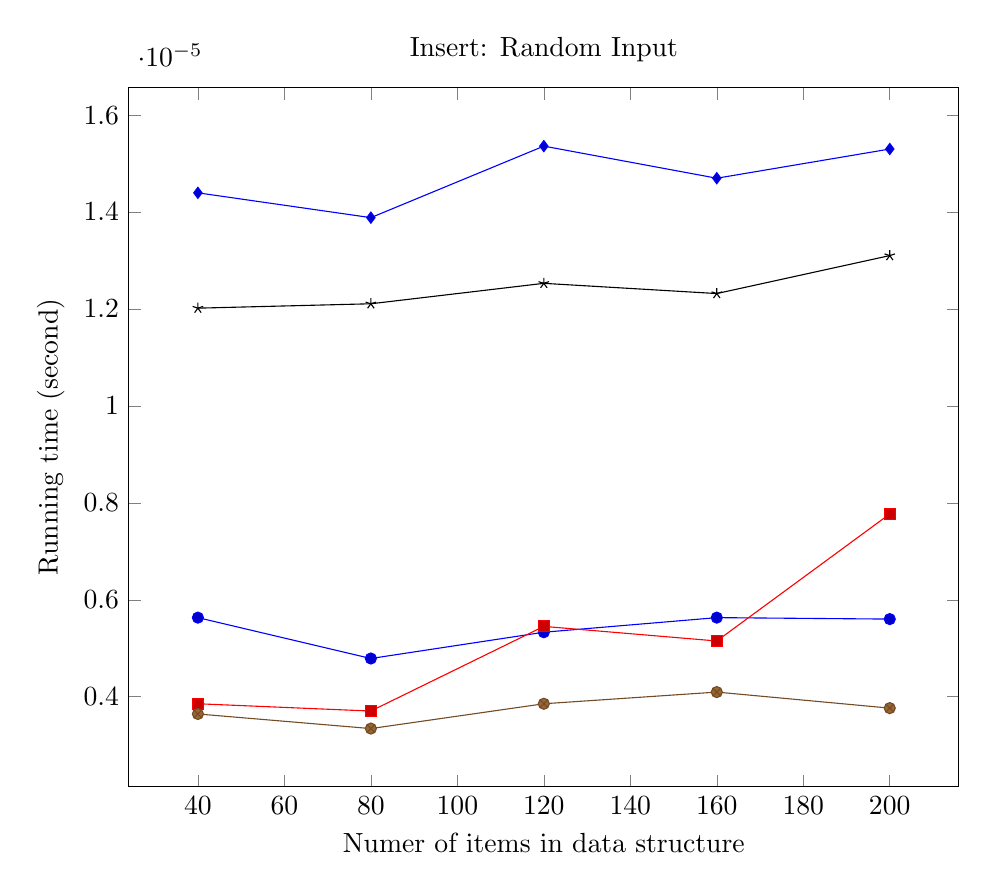
\begin{tikzpicture}
        \begin{axis}[
            xlabel={Numer of items in data structure},
            ylabel={Running time (second)},
            title={Insert: Random Input},
            width=\textwidth
        ]
		\addplot coordinates {
			(200, 5.601861263571095e-06)
			(160, 5.6319787972824996e-06)
			(120, 5.330803460523726e-06)
			(80, 4.7886878544289855e-06)
			(40, 5.6319787972824996e-06)
		};
		\addplot coordinates {
			(200, 7.770323688305324e-06)
			(160, 5.15009825861057e-06)
			(120, 5.4512735953693435e-06)
			(80, 3.704456641884235e-06)
			(40, 3.855044310441258e-06)
		};
		\addplot coordinates {
			(200, 3.7646917096623154e-06)
			(160, 4.095984579777223e-06)
			(120, 3.855044310441258e-06)
			(80, 3.343046238057923e-06)
			(40, 3.644221574816697e-06)
		};
		\addplot coordinates {
			(200, 1.3101127148473779e-05)
			(160, 1.2318071273043073e-05)
			(120, 1.2528894009022907e-05)
			(80, 1.2107248537418513e-05)
			(40, 1.2016895936639571e-05)
		};
		\addplot coordinates {
			(200, 1.5299707106919415e-05)
			(160, 1.4697356433401865e-05)
			(120, 1.5359942174342223e-05)
			(80, 1.3884183024259756e-05)
			(40, 1.439618109664309e-05)
		};
        \legend{}
        \end{axis}
    \end{tikzpicture}
    \caption{Average of 0 operations, benchmarked every 0, starting at 0.}
\end{figure}